\documentclass[10pt,a4paper]{scrartcl}

\usepackage[utf8x]{inputenc}
\usepackage{ucs}
\usepackage{amsmath}
\usepackage{amsfonts}
\usepackage{amssymb}
\usepackage{subfig}
\usepackage{graphicx}


\author{Simon Wallner\\\texttt{me@simonwallner.at}}
\title{HCC Project Seminar - Project Proposal}
\subtitle{project working title: \emph{Sputnik}}


\begin{document}
\maketitle

\begin{abstract}
This project is about using a motion controller as a \emph{New Interface for Musical Expression} (\emph{NIME}). It is used to manipulate sound creating objects in a 3D Scene. The final system should be capable of making use of bigger as well as smaller motions and fine nuances to articulate the performers expression.
\end{abstract}

\section{Introduction}
The system is designed to work with a motion controller like the \emph{Wii Remote} controller. Interaction with the virtual scene is visualized as an elastic \emph{light arc} that seems to be coming out of the controller and reaches into the scene. The endpoint of the arc is fixed at the object the user interacts with. The arc now follows the motions of the controller as if it were a long and elastic fishing rod.

This metaphor should be immediately comprehensible also for uninformed users and users that are not familiar with the input device.  Figure \ref{fig:motion} illustrates the interaction.


\begin{figure}[hbtp]
\centering
\subfloat[bigger motion]{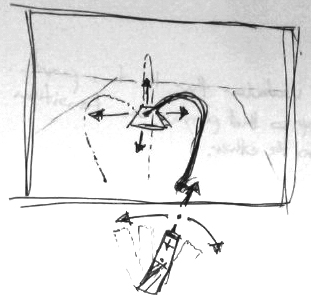
\includegraphics[width=0.4\columnwidth]{img/move}}
\subfloat[finer motion]{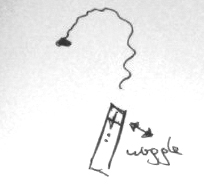
\includegraphics[width=0.4\columnwidth]{img/waggle}}
\caption{Bigger motions are used to apply a pulling force to objects in the scene while finer motions can be used for finer effects like vibrato, etc.}
\label{fig:motion}
\end{figure}

\section{Interaction}
The user interacts with the scene through this arc of light. The body is extended into the scene. Interaction occurs on three layers:

\begin{description}
\item[bigger motions] The primary interaction is to apply a pulling force to objects. Movable objects can be dragged around the scene. This is the domain of the arm and the whole body.

\item[finer motions] The second interaction layer comes from finer motions like a slight wiggle of the controller or a subtle rotation. This is what enables fine artistic expression. It is the domain of the hand and the fingers. Like the vibrato of violin player. 

\item[buttons] The final layer are simple button presses, that can be used as well.
\end{description}

\section{Scientific Merit}
During my quick research I didn't find any work that concentrated on the extension of the body into the virtual scene and on the fine motions required for true artistic expression. My search was generally influence by \cite{Dobrian2006} which emphasises the importance of expression and virtuosity in new music interfaces.

\bibliographystyle{apalike}
\bibliography{library}

\end{document}